%-----------------------------------------------------------------
%	INTRODUCCIÓ
%	!TEX root = ./../main.tex
%-----------------------------------------------------------------
\section{Introducció}
\subsection{Història}
% WIP: 7 wanderers
La setmana té set dies perquè, abans de la invenció del telescopi, es veien set objectes movent-se per l'esfera celeste: els 7 astres errants o planetes, com els hi anomenaven els antics. A cadascun li correspon un dia de la setmana: la Lluna, Mart, Mercuri, Júpiter, Venus, Saturn, i el Sol.

Abans de l'ús del telescopi en l'astronomia, aquesta es va concentrar en estudiar la posició i moviment dels cossos celestes, formats suposadament per la quinta essència.

No obstant, la llei de la gravitació (Newton), l'estudi de les ratlles espectrals, i la composició dels meteorits ens confirmen que la naturalesa dels cossos celestes extraterrestres no difereix essencialment dels terrestres, eliminant la necessitat de la quinta essència.

\subsubsection*{Moviment dels astres: epicicles}
L'epicicle és un dels elements geomètrics bàsics del sistema geocèntric de Claudi Ptolemeu, basat en un Terra que ocupa el centre de l'Univers.
\begin{figure}[h]
	\centering
	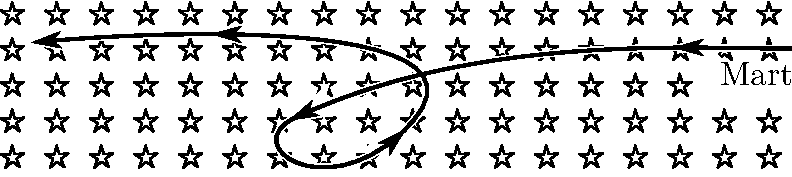
\includegraphics[width=0.7\textwidth]{./images/1-epicycles-a}
	% \textcolor{gray}{\rule{8cm}{4cm}}
	\caption{Problema dels epicicles}
	\label{fig:epicycles-a}
\end{figure}

La teoria dels epicicles va ser dissenyada per Apol·loni de Pèrgam a finals del segle III aC i perfeccionada posteriorment per Ptolemeu. En aquest model, per explicar les variacions de velocitat i direcció del moviment aparent dels planetes, tots els cossos celestes es mouen al voltant de la Terra en cercles petits, anomenats \textit{epicicles}, que al seu torn, es mouen sobre cercles majors anomenats \textit{deferents}. Són els cercles deferents els que estan centrats a la Terra. Ptolemeu, a més, per explicar més precisament els moviments planetaris, va introduir el punt \textit{equant} i va desplaçar el centre del cercle deferent del centre de la Terra.
\begin{figure}[H]
	\centering
	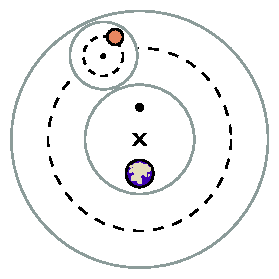
\includegraphics[width=0.3\textwidth]{./images/1-epicycles-b}
	\caption{Elements bàsics del sistema planetari de Claudi Ptolemeu}
	\label{fig:epicycles-b}
\end{figure}

% FIXME: copernicus@sec:bio
L'antiga concepció dels epicicles va ser eliminada amb el desenvolupament de la teoria heliocèntrica de Nicolau Copèrnic (1473--1543) i l'explicació del moviment planetari en òrbites el·líptiques va ser donada per Johannes Kepler.

Tant el telescopi òptic, el descobriment de les ratlles espectrals, el radiotelescopi, així com l'aplicació de la física i les matemàtiques a l'estudi dels cossos celestes van suposar avenços especialment notables, com ara:
\begin{itemize}
	\item Naturalesa i evolució de les estrelles i els seus estats finals (nana blanca, estrella de neutrons, forats negres).
	\item Galàxies més enllà de la Via Làctia.
	\item Expansió de l'Univers.
	\item Radiació de fons de microones.
	\item Expansió accelerada de l'Univers.
\end{itemize}

\subsubsection*{Aberració estel·lar}
% FIXME: bradley@sec:bio
La descripció de l'aberració estel·lar per James Bradley (1728) va confirmar per primer cop la teoria heliocèntrica de Copèrnic.

S'entén per aberració estel·lar la petita diferència angular entre la posició aparent d'una estrella al firmament i la seva vertadera posició.

Aquest fenomen es deu a l'efecte conjunt del moviment de l'observador terrestre i el fet que la velocitat de la llum és finita. El desplaçament (en la posició) i la seva direcció depenen de la velocitat de l'observador i de la seva direcció de moviment.
\begin{figure}[h]
	\centering
	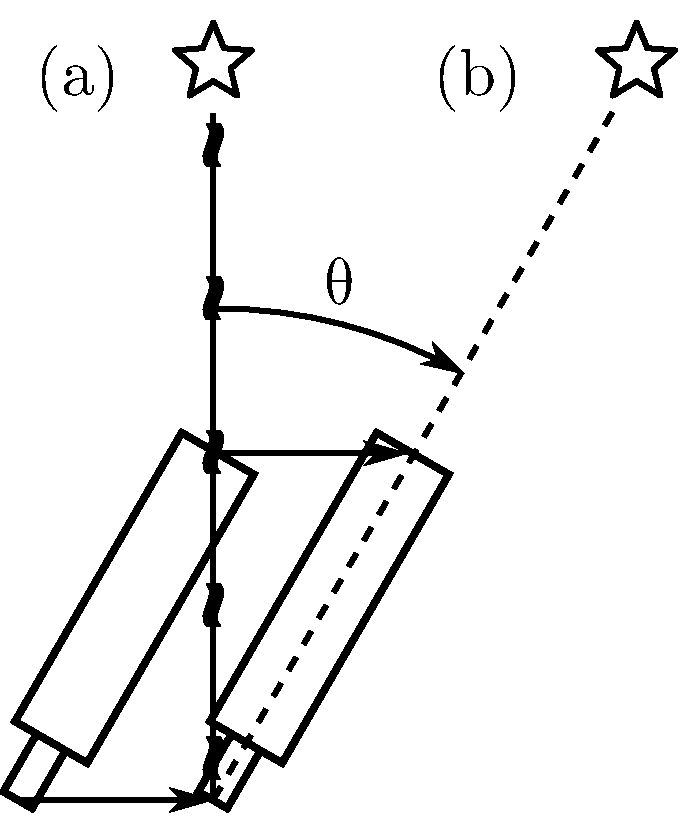
\includegraphics[width=0.3\textwidth]{./images/1-aberration}
	\caption{Aberració estel·lar deguda al moviment de la Terra, on (a) és la font de llum real, i (b) és la font de llum aparent}
	\label{fig:aberration}
\end{figure}
\begin{figure}[h]
	\centering
	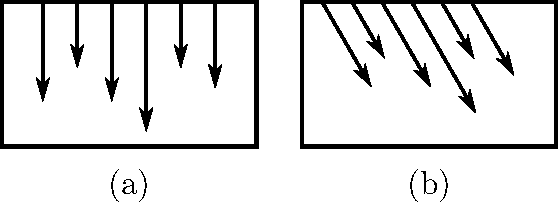
\includegraphics[width=0.45\textwidth]{./images/1-aberration-analogy}
	\caption{Analogia de l'aberració estel·lar amb un cotxe en moviment: (a) cotxe en repòs, (b) cotxe en moviment}
	\label{fig:aberration-analogy}
\end{figure}

L'aberració anual es deu al moviment orbital de la Terra en torn al Sol. Existeix, a més a més, l'\textit{aberració diürna} (molt més petita) deguda a la rotació de la Terra en torn al seu eix.

L'aberració és més fàcilment advertida per a estrelles llunyanes a l'eclíptica. Bradley va trobar aberracions de quasi $\SI{20.5}{\arcsecond}$ al pol celeste. És immediat veure que
\begin{align}
	\tan \theta = \frac{v}{c}
\end{align}
cosa que va permetre a Bradley a determinar la velocitat de la llum amb un error de només el $\SI{2}{\percent}$.

Coneguda la velocitat de la llum, la relació anterior permet esbrinar la velocitat mitjana orbital de la Terra:
\begin{align*}
	v = c \tan(\Delta \theta_{\max}) = \SI{3 e5}{\km \per \s} \tan(\SI{20.5}{\arcsecond}) \approx \SI{29.8}{\km\per\s}
\end{align*}
Bradley, doncs, va confirmar per primera vegada les idees de Copèrnic i Galileu que la Terra orbita en torn al Sol (i no del revés).
\begin{example}
	Si es coneix el producte $G \Msun$, la distància (mitjana) Terra--Sol es pot determinar mitjançant
	\begin{align*}
		d = \frac{G \Msun}{v^{2}} = \SI{1.49 e13}{\cm} \equiv \SI{1}{\au}
	\end{align*}
\end{example}

\subsubsection*{Mètode}
El mètode de l'astrofísica consisteix en observació (telescopi, radiotelescopi, interferòmetre, espectrògraf, etc.) juntament amb teoria.

Pot ser útil considerar la següent analogia: la nostra observació de l'Univers (a escala temporal) seria equivalent a una nau extraterrestre observant la Terra en la seva òrbita durant uns 2 minuts.

%-----------------------------------------------------------------
\subsection{Contingut de l'Univers}
A primera vista predominen les estrelles de massa $\SI{0.08}{\Msun} \lesssim M \lesssim \SI{100}{\Msun}$ aïllades (freqüentment) o en grups. L'estrella més propera al Sol és Proxima Centauri [\href{http://apod.nasa.gov/apod/ap051204.html}{APOD~051204}], situada a $\approx \SI{4.24}{\lightyear}$.

Hi ha una gran varietat en massa, mida, i lluminositat. Sírius, una estrella doble de la constel·lació del Can, és la més brillant amb una magnitud aparent de $m = -1.46$ [\href{http://apod.nasa.gov/apod/ap000611.html}{APOD~000611}].

\subsubsection*{Medi interestel·lar}
El medi interestel·lar està format per
\begin{itemize}
	\item Núvols de gas i pols de molt baixa densitat.
	\item Raigs còsmics girant en camps magnètics.
	\item Regions H II (e.g., nebulosa del Cranc [\href{http://apod.nasa.gov/apod/ap130905.html}{APOD\footnote{\textit{Astronomy Picture of the Day} (APOD) és un lloc web proporcionat per la NASA i la Universitat Tecnològica de Michigan (MTU). Segons el lloc web, «\textit{Cada dia una imatge diferent o fotografia del nostre Univers apareix, juntament amb una breu explicació escrita per un astrònom professional}». La sintàxi de les entrades del web és \url{http://apod.nasa.gov/apod/apYYMMDD.html}.} 130905}]).
	\item Nebuloses planetàries (e.g., nebulosa de l'Ull de Gat [\href{http://apod.nasa.gov/apod/ap141109.html}{APOD~141109}]).
\end{itemize}

\subsubsection*{Cúmuls estel·lars}
Els grups d'estrelles s'anomenen núvols o cúmuls (clústers) estel·lars. En podem trobar dels següents tipus:
\begin{itemize}
	\item Open clusters $\sim 10^{5}$ estrelles (e.g., Plèiades [\href{http://apod.nasa.gov/apod/ap120903.html}{APOD~120903}]).
	\item Globular clusters $\sim 10^{6}$ estrelles (e.g, estrelles velles).
\end{itemize}
Els cúmuls formen, en conjunt, estructures estel·lars que anomenem supercúmuls (superclusters) (e.g., Coma Supercluster [\href{http://apod.nasa.gov/apod/ap080616.html}{APOD~080616}]).

\subsubsection*{Galàxies}
Són sistemes de $\sim \numrange{e10}{e12}$ estrelles. La Via Làctia pertany al Grup Local (format per més de 54 galàxies, essent la majoria d'elles galàxies nanes).

La Galàxia d'Andròmeda [\href{http://apod.nasa.gov/apod/ap140730.html}{APOD~140730}], a uns $\SI{2}{\mega \lightyear}$ i amb una extensió de $\SI{e5}{\lightyear}$, és la més prominent del Grup Local.

\subsubsection*{Regions H I}
Reben aquest nom núvols molt tènues d'àtoms neutres d'hidrogen en zones interestel·lars. Aquests núvols orbiten en torn al centre de la Galàxia amb velocitat dependent de la distància al centre de la mateixa.

Van ser detectades gràcies al fotó en la transició paral·lel$\to$antiparal·lel dels espins del protó i l'electró de l'àtom. La diferència d'energia entre ambdues configuracions és minúscula ($\Delta E = \SI{6 e-6}{\eV}$). Per això, la longitud d'ona del protó emès sigui aproximadament d'un pam:
\begin{align}
	\lambda = \frac{hc}{\Delta E} = \SI{21.2}{\cm}
\end{align}
Aquesta transició paral·lel--antiparal·lel és poc freqüent, ja que la seva probabilitat és molt baixa ($\approx \SI{2.7 e-15}{\per\s}$).

A l'any 1945, van de Hulst va predir que ones de ràdio de la corresponent freqüència ($\SI{1.40 e9}{\Hz}$) podrien ser detectades, les quals serien indicis de l'existència de les regions H I. Els àtoms en elles estarien al seu nivell fonamental d'energia i formarien un gas fred (entre 10 i 100 kelvin).

La mida dels núvols varia entre 1 i 10 parsecs; el nombre d'àtoms per centímetre cúbic, entre 1 i 100.

Gràcies a l'existència d'aquestes regions, amb l'ajuda de radiotelescopis s'ha pogut conèixer (en bona part) l'estructura de la Galàxia.

\subsubsection*{Altres}
\begin{itemize}
	\item Matèria fosca.
	\item Bany de radiació còsmica a $\SI{2.7}{\K}$ (CBM): COBE, WMAP, Planck (vegeu la figura \ref{fig:wmap-planck}).
	\item Bany de neutrins.
	\item Ones gravitacionals: \textit{Laser Interferometer Space Antenna} (LISA, \url{http://lisa.nasa.gov/}).
\end{itemize}
\begin{figure}[H]
	\centering
	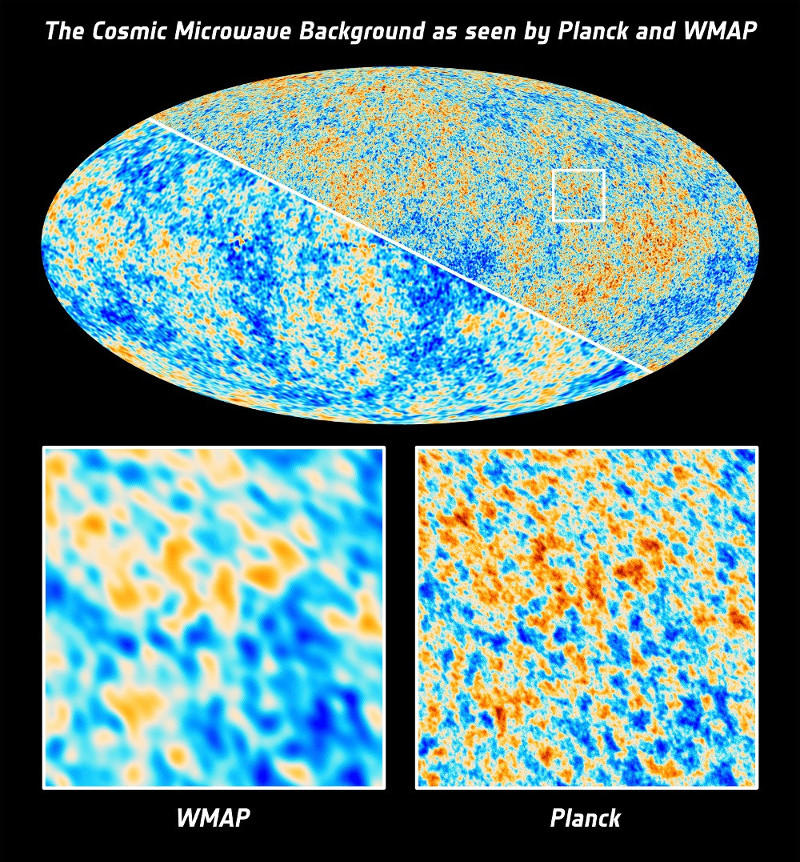
\includegraphics[width=0.7\textwidth]{./images/1-wmap-planck}
	\caption{Comparació de la capacitat de resolució del WMAP (2001) i del \textit{Planck Satellite} (2009) de la radiació còsmica de fons}
	\label{fig:wmap-planck}
\end{figure}

%-----------------------------------------------------------------
\subsection{Instrumentació}
\subsubsection*{Telescopi òptic}
Un telescopi és un sistema òptic que permet veure objectes llunyans, tot ampliant-ne la seva mida angular i la seva lluminositat aparents. Probablement els telescopis són l'eina més important en astronomia i astrofísica. Tot i que amb la paraula \textit{telescopi} hom s'acostuma a referir als telescopis òptics, hi ha telescopis per a gairebé totes les freqüències de l'espectre electromagnètic.

Tot telescopi òptic està format per un objectiu i un ocular. L'objectiu forma una imatge (normalment real) de l'objecte llunyà sobre el seu pla focal; aquesta imatge és llavors ampliada per l'ocular o bé impressionada sobre una pel·lícula fotogràfica o detectada per una càmera CCD (\textit{charge-coupled device}). Si l'objectiu és una lent es parla de telescopi refractor, si l'objectiu és un mirall còncau es parla de telescopi reflector; si utilitza una combinació de lents i miralls s'anomena telescopi catadiòptric.
\begin{figure}[h]
	\centering
	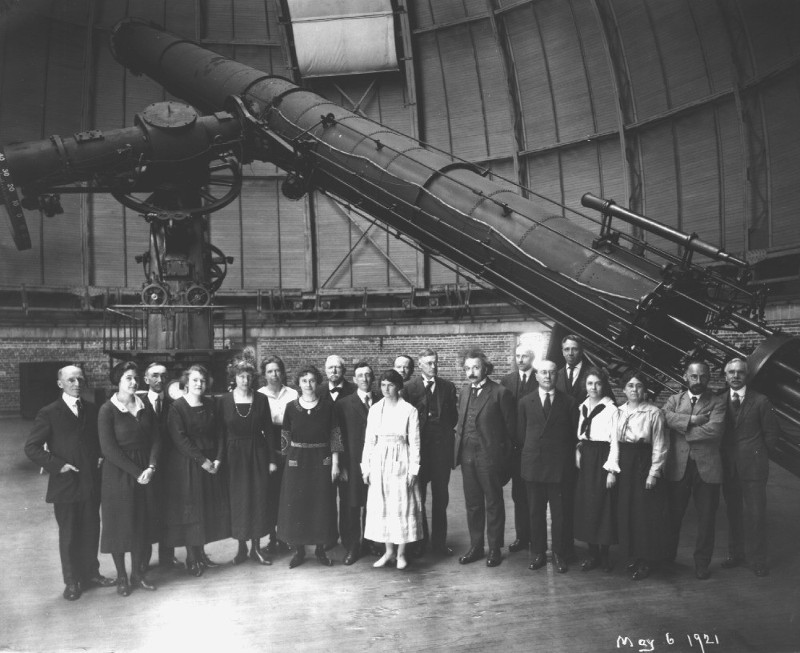
\includegraphics[width=0.6\textwidth]{./images/1-yerkes}
	\caption{Albert Einstein a l'Observatori Yerkes el 6 de maig de 1921}
	\label{fig:yerkes}
\end{figure}

% FIXME: hale@sec:bio
L'Observatori Yerkes (figura \ref{fig:yerkes}) és un observatori astronòmic operat per la Universitat de Chicago. L'observatori, que s'autodenomina \textit{el lloc de naixement de l'astrofísica moderna} va ser fundat al 1897 per George Hale i finançat per Charles Yerkes. Va representar un canvi en la manera de pensar sobre els observatoris, des de ser un mer habitatge per als telescopis i els observadors, a la concepció moderna de l'equip d'observació integrat amb espai de laboratori per a la física i la química.

% FIXME: hubble@sec:bio
% FIXME: chandra@sec:bio
L'observatori té el major telescopi refractor del món utilitzat amb èxit per l'astronomia i una col·lecció de més de 170,000 plaques fotogràfiques. Astrònoms notables han dut a terme investigacions al Yerkes, com ara Edwin Hubble (que va fer el seu treball de postgrau al Yerkes i per a qui el \textit{Hubble Space Telescope} va ser nomenat), Subrahmanyan Chandrasekhar (per a qui el \textit{Chandra Space Telescope} va ser nomenat), el prolífic astrònom rus-americà Otto Struve, i el famós divulgador de l'astronomia Carl Sagan.

\subsubsection*{Radiotelescopi}
Karl Jansky (1931) va descobrir senyals de ràdio de més enllà del Sistema Solar, fonamentalment de la constel·lació de Sagitari. Aquest descobriment va marcar el naixement de la radioastronomia.

Els senyals de ràdio s'originen en la interacció de partícules carregades amb camps electromagnètics.
La unitat que s'utilitza per mesurar la densitat de flux espectral és el Jansky. En particular, al CGS, $\SI{1}{\jansky} = \SI{e-3}{\erg \per \square\m \per \Hz}$.

El disc d'un radiotelescopi reflexa a una antena l'energia de les ones rebudes de la font extraterrestre. A continuació el senyal és amplificat i processat donant lloc a un ràdio-mapa del cel a la longitud d'ona en qüestió.

\subsubsection*{Criteri de Rayleigh}
El criteri de Rayleigh especifica la separació mínima entre dues fonts de llum que es poden resoldre en dos objectes diferents.
\begin{align}
	D \approx 1.22\frac{\lambda}{\theta}
\end{align}
\begin{example}
	Si $\lambda = \SI{21}{\cm}$ (corresponent a una regió H I, per \textit{spin-flip}), per obtenir una resolució de $\SI{1}{\arcsecond} = \SI{4.85 e-6}{\radian}$, caldria un radiotelescopi de diàmetre
	\begin{align*}
	D \approx 1.22 \frac{0.21}{4.85\times 10^{6}} \approx \SI{52.82}{\km}
	\end{align*}
	No obstant això, observem que radiotelescopis moderns com ara del Arecibo Observatory [\href{http://apod.nasa.gov/apod/ap981129.html}{APOD~981129}], té un diàmetre de $D = \SI{300}{\m}$.
\end{example}

\subsubsection*{Interferometria}
\begin{figure}[h]
	\centering
	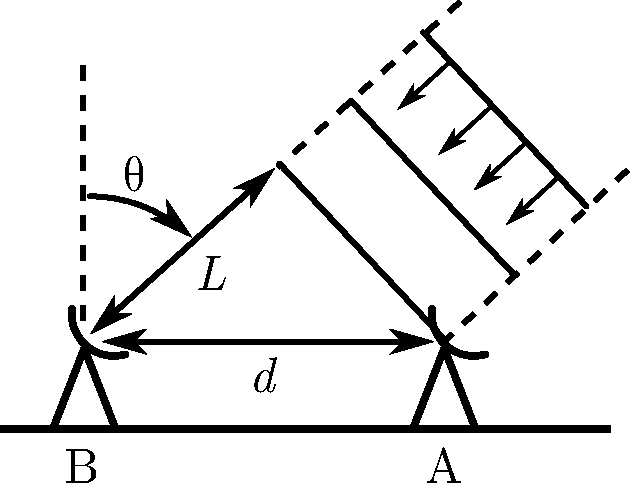
\includegraphics[width=0.3\textwidth]{./images/1-interferometry}
	\caption{Diagrama simplificat de la tècnica de radiointerferometria}
	\label{fig:interferometry}
\end{figure}
Per obtenir una resolució suficient es recorre a l'interferometria, fent ús de dos o més radiotelescopis. Les ones estan en fase si
\begin{align}
	\begin{cases} L = n \lambda & \text{(màxim)}\\ L = \qty(n - \dfrac{1}{2}) \lambda & \text{(mínim)} \end{cases}
\end{align}
ja que $\sin \theta = \dfrac{L}{d}$. Llavors, es pot determinar amb una molt bona aproximació la posició de la font. Actualment, s'aconsegueixen resolucions de la mil·lèsima de segons d'arc.


El VLA (\textit{Very Large Array}), localitzat a Nou Mèxic, és un conjunt de 27 radiotelescopis disposats en $Y$ sobre rails. Tenen un diàmetre de $D = \SI{25}{\m}$. El senyal de cada radiotelescopi és combinat amb la resta i analitzat mitjançant un ordinador per, finalment, produir un ràdio-mapa d'alta resolució del cel.
\begin{figure}[h]
	\centering
	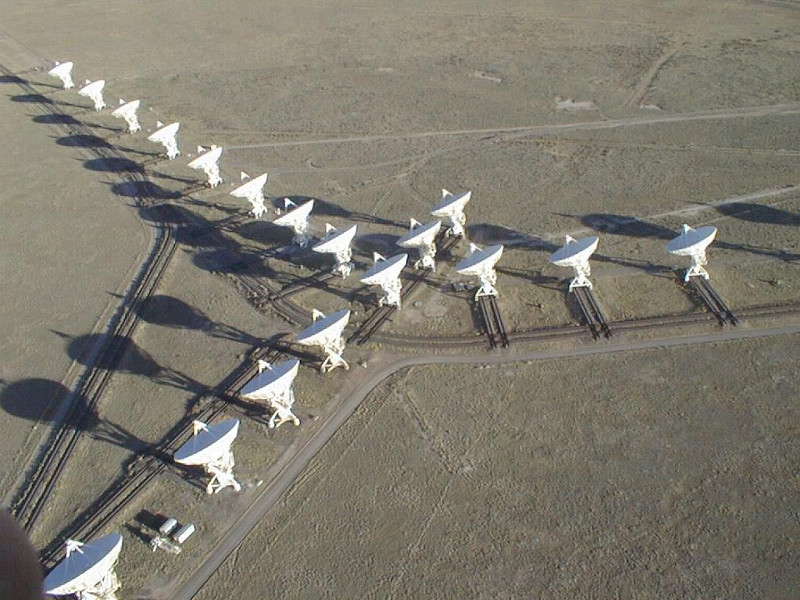
\includegraphics[width=0.6\textwidth]{./images/1-vla}
	\caption{Fotografia del \textit{Very Large Array}}
	\label{fig:vla}
\end{figure}

%-----------------------------------------------------------------
\subsection{Finestres observacionals}
Per a longituds d'ona fora de l'espectre visible i de ràdio, l'atmosfera es mostra opaca (en diversa mesura) a la radiació electromagnètica (figura \ref{fig:observational-windows}).
\begin{figure}[H]
	\centering
	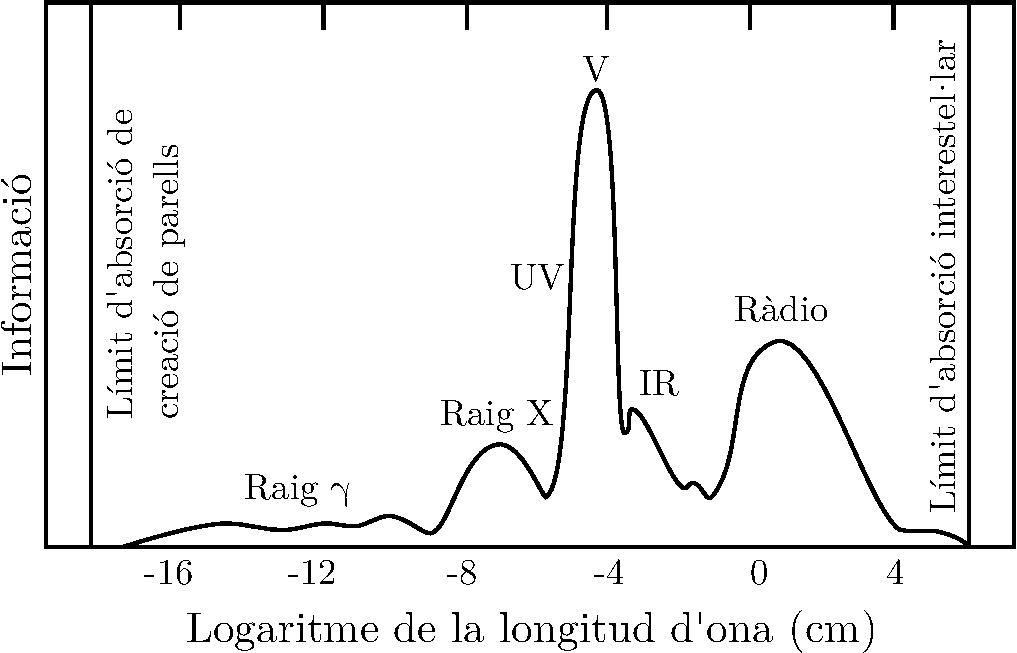
\includegraphics[width=0.65\textwidth]{./images/1-observational-windows}
	\caption{Informació obtinguda mitjançant l'observació en diferents regions de l'espectre electromagnètic}
	\label{fig:observational-windows}
\end{figure}

\subsubsection*{Zona infraroja}
\begin{itemize}
	\item El vapor d'aigua absorbeix la major part de la radiació infraroja.
	\item Mauna Kea (situat a \SI{4205}{\m} sobre el nivell del mar) és un volcà que, per la seva localització, és un lloc ideal per fer observacions d'infrarojos. De fet el \textit{Canada--France--Hawaii Telescope} (CFHT) és el millor telescopi terrestre d'IR en termes resolució d'imatge.
	\item Globus i satèl·lits.
	\item El telescopi i els instruments annexos han de ser refredats suficientment per evitar que la seva emissió IR contamini el senyal extraterrestre (a $\SI{300}{\K} \Rightarrow \lambda \approx \SI{10}{\micro\m})$ .
	\item \textit{Infrared Astronomy Satellite} (IRAS) (1983): $\SI{10}{\micro\m} \lesssim \lambda \lesssim \SI{12}{\micro\m}$, ha detectat pols orbitant estrelles joves, el que suggereix possible formació de planetes.
\end{itemize}

\subsubsection*{Zona de microones}
\begin{itemize}
	\item \textit{Cosmic Background Explorer} (COBE) (1989): \url{http://lambda.gsfc.nasa.gov/product/cobe/}.
	\item \textit{Wilkinson Microwave Anisotropy Probe} (WMAP) (2001): \url{http://map.gsfc.nasa.gov/}.
	\item \textit{Planck Satellite} (2009): \url{http://www.esa.int/Our_Activities/Space_Science/Planck}.
\end{itemize}

\subsubsection*{Zona ultraviolada}
\begin{itemize}
	\item \textit{International Ultraviolet Explorer} (IUE) (1978): $\SI{1200}{\angstrom} < \lambda$.
	\item \textit{Extreme Ultraviolet Explorer} (EUVE) (1992): $\SI{60}{\angstrom} \leq \lambda \leq \SI{740}{\angstrom} \Rightarrow$ informació sobre nanes blanques i púlsars.
\end{itemize}

\subsubsection*{Zona de raigs $X$}
\begin{itemize}
	\item \textit{Röntgensatellit} (ROSAT) (1990): $\SI{5.1}{\angstrom} \leq \lambda \SI{124}{\angstrom} \Rightarrow$ informació sobre quàsars i estrelles de neutrons.
	\item \textit{Chandra X-Ray Observatory} (CXO) (1999) \url{http://www.nasa.gov/mission_pages/chandra/main/}.
\end{itemize}

\subsubsection*{Zona de raigs $\gamma$}
\begin{itemize}
	\item \textit{Compton Gamma Ray Observatory} (CGRO) (1991) té quatre diferents detectors amb energies als intervals
	\begin{align*}
	\begin{aligned}
		\SI{20}{\keV} &\leq E_{\gamma} \leq \SI{600}{\keV} \\
		\SI{100}{\keV} &\leq E_{\gamma} \leq \SI{10}{\MeV} \\
		\SI{1}{\MeV} &\leq E_{\gamma} \leq \SI{30}{\MeV} \\
		\SI{20}{\MeV} &\leq E_{\gamma} \leq \SI{30}{\GeV} \quad \text{(EGRET).} \\
	\end{aligned}
	\end{align*}
\end{itemize}

\begin{table}[H]
	\centering
		\begin{tabularx}{0.9\textwidth}{cX}
		\toprule
		Longitud d'ona & Objecte característic \\
		\midrule
		Raig Gamma & Objectes compactes en col·lisió (estrelles de neutrons, ...)? \\
		Raig $X$ & Estrelles de neutrons \\
		Ultraviolat & Estrelles calents, quàsars \\
		Visible & Estrelles \\
		Infraroig & Gegants vermelles, nuclis galàctics \\
		IR llunyà & Protoestrelles, pols estel·lar, planetes \\
		Mil·límetre & Pols fred, núvols mol·leculars \\
		Ràdio de \si{\cm} & Línia H I \SI{21}{\cm}, púlsars \\
		\bottomrule
		\end{tabularx}
	\caption{Comparació dels fenòmens característics que són estudiats a diferents longituds d'ona}
	\label{tab:wavelenghts}
\end{table}
